\documentclass[preprint,12pt,aps,pra,showkeys,amsmath,amssymb,superscriptaddress,floatfix]{revtex4-2}
\usepackage[T1]{fontenc}
\usepackage[utf8]{inputenc}
\usepackage{amsmath,amssymb,amsthm,mathtools,mathrsfs}
\usepackage{microtype,booktabs,enumitem}
\usepackage{xcolor,tikz,etoolbox}
\usepackage[skins,breakable]{tcolorbox}
\usepackage{needspace}
% Keep diagram geometry independent of REVTeX preprint body spacing.
\AtBeginEnvironment{tikzpicture}{\linespread{1}\selectfont}
\usetikzlibrary{arrows.meta,positioning,calc,fit,decorations.pathreplacing}
\usepackage{graphicx}
\usepackage{hyperref}

\definecolor{MMBlue}{RGB}{0,82,155}
\definecolor{MMOrange}{RGB}{200,80,0}
\tikzset{
 mmnode/.style={draw=MMBlue,rounded corners=2pt,fill=MMBlue!4,align=left,execute at begin node={\raggedright},text width=5cm,font=\fontsize{10}{12}\selectfont,inner sep=6pt},
 mmimport/.style={mmnode,draw=black!65,fill=black!4},
 mmcandidate/.style={mmnode,draw=MMOrange,dashed,fill=MMOrange!5},
 mmrejected/.style={mmnode,draw=black,densely dotted,fill=black!8},
 mmproof/.style={->,thick,MMBlue},
 mmflow/.style={->,semithick,black!70},
 mmrepair/.style={->,dashed,thick,MMOrange},
 mmcandidatearrow/.style={->,dashed,semithick,MMOrange},
 mmnote/.style={font=\scriptsize,fill=white,inner sep=2pt,align=center}}

\usepackage[section]{placeins}
\setlength{\emergencystretch}{3em}
\setlist{itemsep=3pt,topsep=4pt}
\newtheorem{theorem}{Theorem}[section]
\newtheorem{proposition}[theorem]{Proposition}
\newtheorem{lemma}[theorem]{Lemma}
\newtheorem{corollary}[theorem]{Corollary}
\theoremstyle{definition}
\newtheorem{definition}[theorem]{Definition}
\newtheorem{example}[theorem]{Example}
\theoremstyle{remark}
\newtheorem{remark}[theorem]{Remark}
% Avoid isolated statement headings and single-line paragraph fragments.
\BeforeBeginEnvironment{theorem}{\Needspace{6\baselineskip}}
\BeforeBeginEnvironment{definition}{\Needspace{5\baselineskip}}
\BeforeBeginEnvironment{proposition}{\Needspace{5\baselineskip}}
\BeforeBeginEnvironment{lemma}{\Needspace{5\baselineskip}}
\BeforeBeginEnvironment{corollary}{\Needspace{5\baselineskip}}
\clubpenalty=5000
\widowpenalty=5000
\newcommand{\R}{\mathbb R}\newcommand{\Z}{\mathbb Z}\newcommand{\N}{\mathbb N}
\newcommand{\Pa}{\operatorname{Pa}}\newcommand{\Desc}{\operatorname{Desc}}
\newcommand{\cl}{\operatorname{cl}}\newcommand{\cost}{\operatorname{cost}}
\newcommand{\status}{\operatorname{status}}
% Faculty cards: a visual rail groups the five faculties within one agent.
% The rail has no arrowhead and does not represent a proof dependency.
\newcommand{\mmfacultybadge}[1]{%
 \node[circle,draw=MMBlue,line width=1pt,fill=white,
 minimum size=7mm,inner sep=0pt,font=\sffamily\small\bfseries,text=MMBlue]
 at ([xshift=15pt,yshift=-15pt]frame.north west) {#1};}
\newcommand{\mmfacultyrail}{%
 \draw[MMBlue!80,line width=1pt]
 ([xshift=15pt,yshift=2pt]frame.north west)--
 ([xshift=15pt,yshift=-2pt]frame.south west);}
\newtcolorbox{mmfacultybox}[2]{enhanced,breakable,
 colback=MMBlue!4,colframe=MMBlue!4,boxrule=0pt,arc=3pt,
 left=39pt,right=9pt,top=4pt,bottom=4pt,
 before skip=2pt,after skip=2pt,
 fontupper=\small\linespread{1.1}\selectfont,
 overlay unbroken={\mmfacultyrail\mmfacultybadge{#1}},
 overlay first={\mmfacultyrail\mmfacultybadge{#1}},
 overlay middle={\mmfacultyrail},overlay last={\mmfacultyrail}}
\newcommand{\mmfaculty}[3]{%
 \begin{mmfacultybox}{#1}{#2}
 {\sffamily\bfseries\color{MMBlue}#2}\par\smallskip #3
 \end{mmfacultybox}}
\newcommand{\agent}[9]{%
 \Needspace{8\baselineskip}
 \subsubsection{#1}
 \noindent\textbf{Object.} #2\par
 \noindent\textbf{Role.} #3\par\smallskip
 \mmfaculty{E}{Ego}{#4}
 \mmfaculty{M}{Memory}{#5}
 \mmfaculty{I}{Intellect}{#6}
 \mmfaculty{S}{Sense}{#7}
 \mmfaculty{A}{Action}{#8}
 \smallskip\noindent #9\par}

\usepackage{longtable,array,calc}
\providecommand{\tightlist}{\setlength{\itemsep}{2pt}\setlength{\parskip}{0pt}}
\makeatletter
\def\frontmatter@abstract@produce{\par\addvspace{\frontmatter@preabstractspace}%
\begingroup\prep@absbox\unvbox\absbox\post@absbox\endgroup
\addvspace{\frontmatter@postabstractspace}}
\makeatother
\newcommand{\field}[2]{\par\smallskip\noindent\textbf{#1.} #2\par}
\setlength{\emergencystretch}{5em}
\AtBeginEnvironment{verbatim}{\small\linespread{1.0}\selectfont}


\hypersetup{colorlinks=true,linkcolor=MMBlue,urlcolor=MMBlue,pdfauthor={Dibakar Sigdel}}

\begin{document}

\title{Riesz Representation in Hilbert Spaces\\[4pt]\large An End-to-End Meta-Math Walkthrough}

\author{Dibakar Sigdel}

\affiliation{Mindverse Computing LLC, Lynnwood, WA 98087, USA}

\date{October 2026}

\begin{abstract}

The kernel has an orthogonal direction that captures every value of the
functional; scaling that direction gives the representing vector. The
report presents the target theorem, declared imports, a dependency
graph, five-faculty node contracts, a continuous proof, a worked
example, and a hypothesis-repair audit. It is an authored mathematical
exposition, not a deployed-agent transcript or a formal proof-assistant
certificate.

\end{abstract}\maketitle\linespread{1.12}\selectfont

\noindent\textbf{FA-03 / Functional Analysis and Measure Theory / Report v1}

\section{Target and import contract}

\begin{theorem}

For a real or complex Hilbert space \(H\) with inner product linear in
its first variable, every bounded linear functional
\(\ell:H\to\mathbb F\) has a unique \(y\in H\) such that
\(\ell(x)=\langle x,y\rangle\) for all \(x\in H\). Also
\(\|\ell\|=\|y\|\).

\end{theorem}

\subsection{Foundations and permitted imports}

Import FA-02: every vector has a unique orthogonal decomposition
relative to a closed linear subspace. Use Cauchy--Schwarz and continuity
of bounded linear maps. The operator norm is
\(\|\ell\|=\sup_{\|x\|\le1}|\ell(x)|\). This is the Hilbert-space Riesz
theorem, not the measure representation theorem on spaces of continuous
functions.

\clearpage\section{Node interaction workflow}

\begin{center}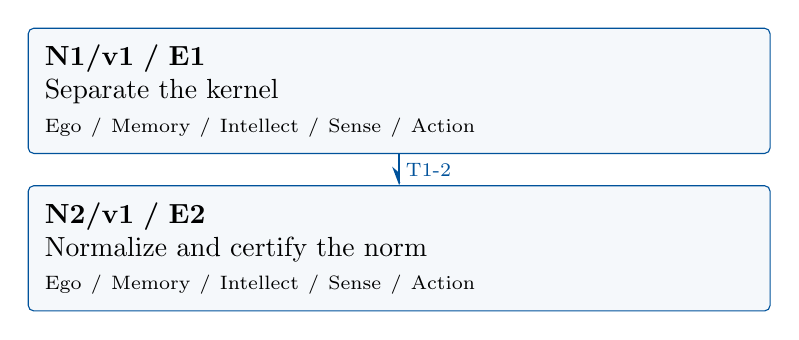
\begin{tikzpicture}[>=Stealth,x=1cm,y=1cm]

\node[mmnode,text width=9cm,minimum height=1.25cm] (N1) at (0,0.0) {\textbf{N1/v1 / E1}\\Separate the kernel\\{\scriptsize Ego / Memory / Intellect / Sense / Action}};

\node[mmnode,text width=9cm,minimum height=1.25cm] (N2) at (0,-2.0) {\textbf{N2/v1 / E2}\\Normalize and certify the norm\\{\scriptsize Ego / Memory / Intellect / Sense / Action}};

\draw[mmproof] (N1.south) -- node[mmnote,right] {T1-2} (N2.north);

\end{tikzpicture}\end{center}

Each box is one mathematical agent containing all five faculties. Blue
arrows carry the versioned exports listed below. The layout gives a
reading order; only drawn arrows assert dependencies. Diagnostic repair
is separate from the proof DAG.

\subsection{Versioned evidence-transfer ledger}

\begingroup\small\linespread{1.05}\selectfont

\Needspace{5\baselineskip}\field{T1-2: N1/E1/v1 to N2}{There is \(z\in K^\perp\) with \(\ell(z)\ne0\), and
\(x-\ell(x)z/\ell(z)\in K\) for every \(x\).}

\field{Receiving activity}{N2.1}

\field{Compatibility}{E1/v1; the first-variable linear convention. Check: The scalar in the
second inner-product argument is conjugated; omitting it changes the
represented functional over \(\mathbb C\).}

\endgroup

\clearpage\section{Agent roles and five-faculty activities}\begingroup\small\linespread{1.05}\selectfont\setlist{itemsep=1pt,topsep=2pt}

\subsection{N1/v1: Separate the kernel}

\field{Object and role}{Project a vector outside the kernel and retain its nonzero perpendicular
remainder. \textbf{Local obligation:} There is \(z\in K^\perp\) with
\(\ell(z)\ne0\), and \(x-\ell(x)z/\ell(z)\in K\) for every \(x\).}

\field{Inputs}{A nonzero bounded functional \(\ell\); its kernel \(K\).}

\mmfaculty{E}{Ego}{Publish E1/v1 only after establishing this obligation: There is
\(z\in K^\perp\) with \(\ell(z)\ne0\), and \(x-\ell(x)z/\ell(z)\in K\)
for every \(x\).}

\mmfaculty{M}{Memory}{A nonzero bounded functional \(\ell\); its kernel \(K\). Retain the
stated assumptions and import versions.}

\mmfaculty{I}{Intellect}{Project a vector outside the kernel and retain its nonzero perpendicular
remainder.}

\mmfaculty{S}{Sense}{The remainder cannot vanish or lie in the kernel, because its functional
value equals the original nonzero value.}

\mmfaculty{A}{Action}{Carry out activities N1.1--N1.2 below, retaining each calculation and
construction as evidence.}

\smallskip\noindent\textbf{Numbered mathematical activities}

\begin{enumerate}[label=N1.\arabic*,leftmargin=3.4em]

\item If \(\ell=0\), take \(y=0\) and the representation and norm equality are
immediate; uniqueness follows from testing the difference against itself
as in N2. For the remaining case choose \(w\) with \(\ell(w)\ne0\).
Continuity makes \(K\) closed, so FA-02 gives \(w=P_Kw+z\) with
\(z\perp K\).

\item Linearity gives \(\ell(z)=\ell(w)\ne0\). For each \(x\), set
\(k=x-\ell(x)z/\ell(z)\). Then \(\ell(k)=0\), so \(k\in K\). Thus
\(\langle x,z\rangle=\ell(x)\|z\|^2/\ell(z)\).

\end{enumerate}

\field{Export E1/v1}{There is \(z\in K^\perp\) with \(\ell(z)\ne0\), and
\(x-\ell(x)z/\ell(z)\in K\) for every \(x\).}

\field{Acceptance gate}{The remainder cannot vanish or lie in the kernel, because its functional
value equals the original nonzero value.}

\field{Targeted repair}{If division by \(\ell(z)\) occurs before nonvanishing is shown, restore
the separate zero-functional case and the equality \(\ell(z)=\ell(w)\).
Withhold this export and recheck its descendants after a versioned
correction.}

\clearpage

\subsection{N2/v1: Normalize and certify the norm}

\field{Object and role}{Choose the conjugate scalar in the second argument, then test at the
normalized representing vector. \textbf{Local obligation:} A unique
\(y\) represents \(\ell\), and \(\|\ell\|=\|y\|\).}

\field{Inputs}{E1/v1; the first-variable linear convention. Incoming proof exports:
E1/v1 at N2.1.}

\mmfaculty{E}{Ego}{Publish E2/v1 only after establishing this obligation: A unique \(y\)
represents \(\ell\), and \(\|\ell\|=\|y\|\).}

\mmfaculty{M}{Memory}{E1/v1; the first-variable linear convention. Incoming proof exports:
E1/v1 at N2.1. Retain the stated assumptions and import versions.}

\mmfaculty{I}{Intellect}{Choose the conjugate scalar in the second argument, then test at the
normalized representing vector.}

\mmfaculty{S}{Sense}{The scalar in the second inner-product argument is conjugated; omitting
it changes the represented functional over \(\mathbb C\).}

\mmfaculty{A}{Action}{Carry out activities N2.1--N2.2 below, retaining each calculation and
construction as evidence.}

\smallskip\noindent\textbf{Numbered mathematical activities}

\begin{enumerate}[label=N2.\arabic*,leftmargin=3.4em]

\item Define \(y=\overline{\ell(z)}z/\|z\|^2\) (drop conjugation over
\(\mathbb R\)). Then
\(\langle x,y\rangle=\ell(z)\langle x,z\rangle/\|z\|^2=\ell(x)\) by E1.

\item If \(y_1,y_2\) represent the same functional,
\(\langle x,y_1-y_2\rangle=0\) for all \(x\). Taking \(x=y_1-y_2\)
proves equality. Cauchy--Schwarz gives \(\|\ell\|\le\|y\|\); if
\(y\ne0\), testing \(x=y/\|y\|\) gives the reverse inequality. The zero
case has both norms zero.

\end{enumerate}

\field{Export E2/v1}{A unique \(y\) represents \(\ell\), and \(\|\ell\|=\|y\|\).}

\field{Acceptance gate}{The scalar in the second inner-product argument is conjugated; omitting
it changes the represented functional over \(\mathbb C\).}

\field{Targeted repair}{If conjugation is absent, recompute the second-argument scalar and check
the one-dimensional complex example before releasing the norm and
representation. Withhold this export and recheck its descendants after a
versioned correction.}

\endgroup\clearpage\section{Continuous mathematical proof}\label{sec:proof}

\subsection{N1 --- Separate the kernel}\label{n1-separate-the-kernel}

\begin{enumerate}
\def\labelenumi{\arabic{enumi}.}
\item
  \textbf{N1.1.} If \(\ell=0\), take \(y=0\) and the representation and
  norm equality are immediate; uniqueness follows from testing the
  difference against itself as in N2. For the remaining case choose
  \(w\) with \(\ell(w)\ne0\). Continuity makes \(K\) closed, so FA-02
  gives \(w=P_Kw+z\) with \(z\perp K\).
\item
  \textbf{N1.2.} Linearity gives \(\ell(z)=\ell(w)\ne0\). For each
  \(x\), set \(k=x-\ell(x)z/\ell(z)\). Then \(\ell(k)=0\), so
  \(k\in K\). Thus \(\langle x,z\rangle=\ell(x)\|z\|^2/\ell(z)\).
\end{enumerate}

\subsection{N2 --- Normalize and certify the
norm}\label{n2-normalize-and-certify-the-norm}

\begin{enumerate}
\def\labelenumi{\arabic{enumi}.}
\item
  \textbf{N2.1.} Define \(y=\overline{\ell(z)}z/\|z\|^2\) (drop
  conjugation over \(\mathbb R\)). Then
  \(\langle x,y\rangle=\ell(z)\langle x,z\rangle/\|z\|^2=\ell(x)\) by
  E1.
\item
  \textbf{N2.2.} If \(y_1,y_2\) represent the same functional,
  \(\langle x,y_1-y_2\rangle=0\) for all \(x\). Taking \(x=y_1-y_2\)
  proves equality. Cauchy--Schwarz gives \(\|\ell\|\le\|y\|\); if
  \(y\ne0\), testing \(x=y/\|y\|\) gives the reverse inequality. The
  zero case has both norms zero.
\end{enumerate}

\hfill$\square$

\section{Worked orchestration}

On \(\mathbb C^2\) with
\(\langle x,y\rangle=x_1\overline{y_1}+x_2\overline{y_2}\), let
\(\ell(x)=x_1+2i x_2\). Its representing vector is \(y=(1,-2i)\), so
\(\|\ell\|=\sqrt5\). The unit vector \(y/\sqrt5\) attains the operator
norm. This checks the conjugation convention directly.

\subsection{Boundary and hypothesis audit}

Completeness matters: on \(c_{00}\) with the \(\ell^2\) norm,
\(\ell(x)=\sum_n x_n/n\) is bounded by Cauchy--Schwarz. A representing
vector within \(c_{00}\) would have coordinates \(1/n\) by testing the
standard basis, an impossibility. The completion \(\ell^2\) supplies
that vector.

\section{Illustrative failure and repair}

The following is an authored diagnostic scenario. Changed assumptions
define a new contract; they do not retroactively prove the original
statement.

\subsection{Rejected argument, diagnosis, and correction}
\textbf{Rejected N2 candidate:} \(y=\ell(z)z/\|z\|^2\) under the
first-variable linear convention. For \(H=\mathbb C\), \(\ell(x)=ix\),
and \(z=1\), it gives \(\langle x,i\rangle=-ix\). \textbf{Diagnosis:}
Memory used the wrong scalar convention. \textbf{Repair:} conjugate
\(\ell(z)\) as in N2.1. The statement is unchanged; recheck both the
representation and its norm certificate.

\subsection{Publication and reuse}
The corrected export retains its explicit assumptions. A hypothetical
revision receives a new version, and each consuming activity is
rechecked; this scenario is not a recorded runtime event. \textbf{Next
direction:} Apply the representation to bounded variational functionals,
as in the weak Poisson existence project.

\par\medskip\begingroup\small\linespread{1.0}\selectfont\noindent\textbf{Provenance.} This authored proof is complete relative to its declared imports. Reuse
each export with its assumptions, proof, and version. The original
Markdown remains available for comparison.
\par\endgroup

\par\smallskip\begingroup\small\linespread{1.0}\selectfont\noindent\textbf{Further reading.} \href{https://ocw.mit.edu/courses/18-102-introduction-to-functional-analysis-spring-2021/resources/lecture-notes/}{MIT
OpenCourseWare, Introduction to Functional Analysis: lecture notes}. See
the lectures on integration, Hilbert spaces, Baire category, and
Hahn--Banach.\par\endgroup

\end{document}
